\newpage
\subsection{Caso d'uso UC2: Main post-autenticazione }
\label{UC2}
\begin{figure}[ht]
	\centering
	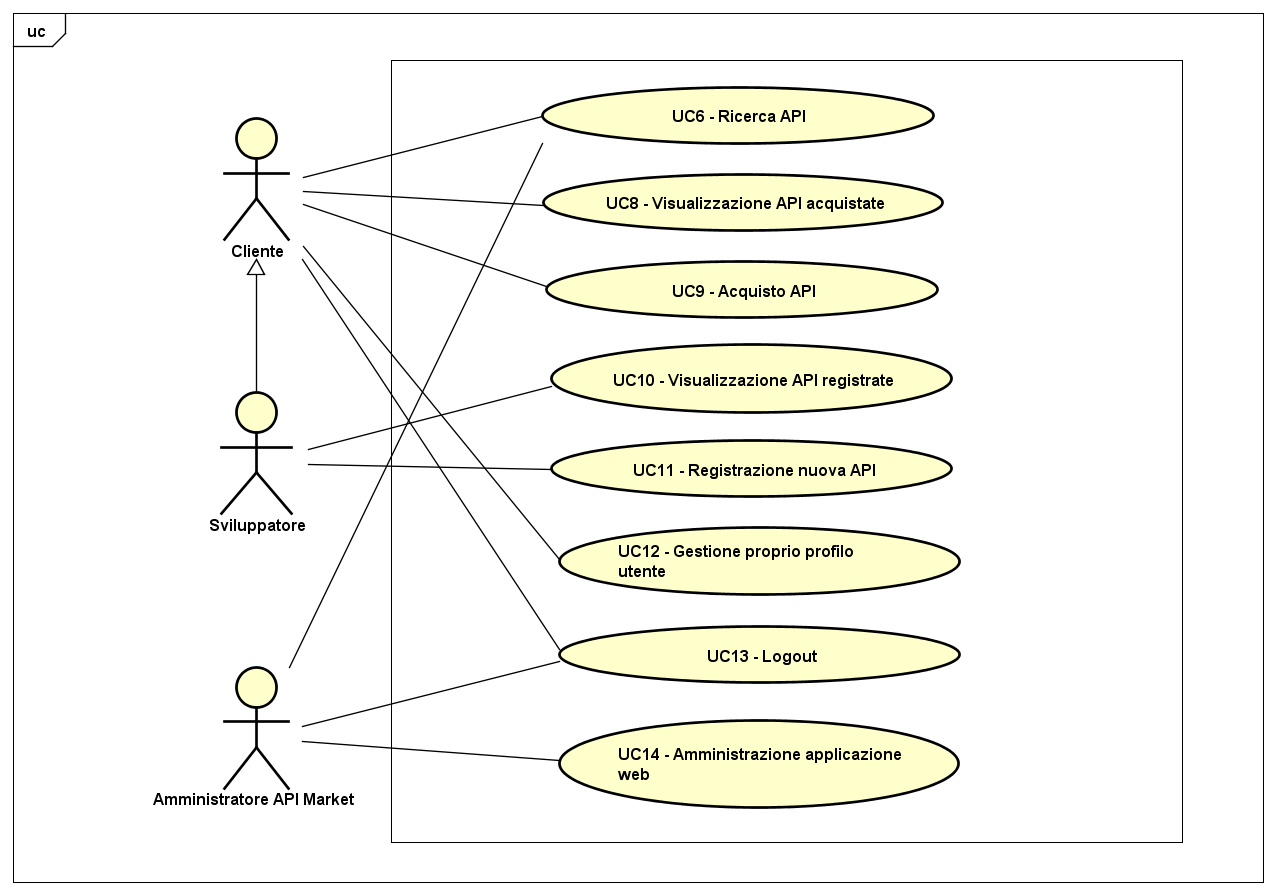
\includegraphics[scale=0.45]{UML/UC2.png}
	\caption{UC2: Main post-autenticazione}
\end{figure}

\begin{longtable}{ l | p{11cm}}
	\hline
	\rowcolor{Gray}
	 \multicolumn{2}{c}{UC2 - Main post-autenticazione} \\
	 \hline
	\textbf{Attori} & Cliente, Sviluppatore, Amministratore API Market \\
	\textbf{Descrizione} & Il cliente, tramite la schermata principale dell'applicazione, può accedere e sfruttare le funzionalità a lui disponibili: la ricerca API, la visualizzazione di API acquistate, l'acquisto API, la gestione del proprio profilo utente, il logout.
	Lo sviluppatore inoltre può visualizzare le API registrate e registrarne di nuove.
	L'amministratore API Market può effettuare una ricerca API ed amministrare l'applicazione web. \\
	\textbf{Pre-Condizioni} & L'attore ha avviato l'applicazione web e si è autenticato. La piattaforma mostra le pagine preposte agli utenti autenticati \\
	\textbf{Post-Condizioni} & L'applicazione ha eseguito le richieste dell'attore \\
	\textbf{Scenario Principale} & 
	\begin{enumerate*}[label=(\arabic*.),itemjoin={\newline}]
		\item L'attore può effettuare una ricerca sulle API presenti nell'applicazione
(UC6)
		\item Il cliente può visualizzare le API da lui acquistate (UC8)
		\item Il cliente può acquistare una API (UC9)
		\item Lo sviluppatore può visualizzare le API da lui registrate (UC10)
		\item Lo sviluppatore può registrare una nuova API (UC11)
		\item Il cliente può gestire il proprio profilo utente (UC12)
		\item L'attore può effettuare il logout (UC13)
		\item L'amministratore API Market può accedere all'amministrazione dell'applicazione web (UC14)
	\end{enumerate*}\\
\end{longtable}